\chapter{Суперзаряды, замыкание и суперпространство}

\lectureoverview{Суперсимметрия трудна не потому, что её правила многочисленны, а потому, что они соединяют идеи, которые обычная физика держит раздельно. Мы начнём с переменных Грассмана, нечётные элементы которых антикоммутируют, а функции от них обрываются после конечного числа членов. Их алгебра производных затем даёт модель для нечётных генераторов симметрии. Бозонный и фермионный осцилляторы дают простейшие суперзаряды: их антикоммутатор есть гамильтониан, так что обмен бозонов и фермионов неотделим от трансляции по времени. Ту же алгебру можно геометрически представить как трансляции по грассмановым направлениям расширенного пространства-времени, называемого суперпространством.}

\section{Почему, прежде чем двигаться дальше, нужно сделать шаг назад}

Суперсимметрия относится к числу самых абстрактных конструкций в физике. Она похожа на вращения и трансляции, поскольку является симметрией, но не помещается в обычное пространство-время, если не расширить само понятие координаты. Её естественные параметры — грассмановы величины: объекты, которые можно складывать и умножать, но которые антикоммутируют, а не коммутируют.

Вот почему прямой переход к окончательной алгебре был бы бесполезен. Сначала мы приведём нечётную арифметику в рабочий вид, затем напомним, как организованы обычные непрерывные симметрии, и лишь потом соединим эти две идеи. Путь длиннее, но каждый шаг подготавливает следующий.

\section{Алгебра Грассмана в рабочем виде}

\subsection{Нечётные и чётные элементы}

Пусть \(\epsilon_i\) обозначают независимые образующие Грассмана. Они удовлетворяют
\begin{equation}
\epsilon_i\epsilon_j=-\epsilon_j\epsilon_i,
\qquad
\{\epsilon_i,\epsilon_j\}=0.
\end{equation}
Полагая \(i=j\), получаем
\begin{equation}
2\epsilon_i^2=0,
\qquad
\epsilon_i^2=0,
\end{equation}
над вещественными или комплексными числами. Каждая образующая не равна нулю; нулю равен только её квадрат.

Каждый однородный элемент имеет чётность. Произведение, содержащее нечётное число образующих Грассмана, нечётно, а произведение, содержащее чётное число, чётно:
\begin{align}
\text{odd}\times\text{odd}&=\text{even},\\
\text{odd}\times\text{even}&=\text{odd},\\
\text{even}\times\text{even}&=\text{even}.
\end{align}
Чётные элементы коммутируют с однородными элементами. Два нечётных элемента антикоммутируют. Поэтому
\begin{equation}
n\epsilon_i=\epsilon_i n,
\qquad
\epsilon_i\epsilon_j=-\epsilon_j\epsilon_i,
\end{equation}
когда \(n\) чётен.

Чётный элемент не обязан быть обычным вещественным или комплексным числом. Произведение \(\epsilon_1\epsilon_2\), например, чётно и нильпотентно. Обычные числа образуют скалярную часть алгебры, а чётные произведения дают дополнительные коммутирующие элементы.

\begin{classroomqa}
\audiencequestion{Есть ли различие между алгеброй Грассмана и числами Грассмана, или это одно и то же? \lecturetimestamp{00:06:45}}
\lecturerresponse{Элементы — это числа Грассмана; алгебра — совокупность этих элементов вместе с правилами их сложения и умножения. Поэтому в нестрогой речи можно иметь в виду один и тот же объект, но полезно различать сами объекты, с которыми работают, и правила, по которым с ними работают.}
\end{classroomqa}

\subsection{Разложения функций конечны}

Функция одной переменной Грассмана имеет только две возможные степени:
\begin{equation}
f(\epsilon)=a+b\epsilon.
\end{equation}
Члена \(\epsilon^2\) нет. Для двух независимых образующих
\begin{equation}
f(\epsilon_1,\epsilon_2)
=a+b_1\epsilon_1+b_2\epsilon_2+c\epsilon_1\epsilon_2.
\end{equation}
Разложение обрывается после того, как появились обе образующие. Для \(n\) независимых образующих упорядоченные мономы образуют базис размерности \(2^n\):
\begin{equation}
1,\quad
\epsilon_i,\quad
\epsilon_i\epsilon_j,\quad
\ldots,\quad
\epsilon_1\epsilon_2\cdots\epsilon_n.
\end{equation}
\editorialnote{Конечномерное утверждение размерности \(2^n\) — это общий образец, лежащий в основе примеров с одной и двумя образующими. Можно определить и бесконечную алгебру Грассмана, но каждый используемый здесь многочлен содержит лишь конечное число образующих.}

Когда две вещественные образующие объединяют в комплексную пару \(\theta,\bar\theta\), общую функцию при выбранном порядке можно записать как
\begin{equation}
f(\theta,\bar\theta)
=a+\bar b\,\theta+\bar\theta\,b+c\,\bar\theta\theta.
\end{equation}
Черта указывает на используемое здесь обозначение комплексной пары. Если поменять порядок в последнем произведении, знак изменится:
\begin{equation}
\bar\theta\theta=-\theta\bar\theta.
\end{equation}

Обычно всей функции удобно приписать определённую чётность. Если \(f\) чётна, то \(a\) и \(c\) чётны, а \(b\) и \(\bar b\) нечётны. Если \(f\) нечётна, эти назначения обращаются. Сами коэффициенты могут принадлежать большей алгебре Грассмана, при условии что они не зависят от тех конкретных переменных, по которым выполняется разложение.

\begin{classroomqa}
\audiencequestion{Можно ли подставить переменную Грассмана в тригонометрические или другие аналитические функции? \lecturetimestamp{00:11:06}}
\lecturerresponse{Да, но степенной ряд обрывается сразу. Для одной нечётной образующей
\[
\sin\epsilon=\epsilon,\qquad
\cos\epsilon=1,\qquad
e^\epsilon=1+\epsilon.
\]
Привычные названия сохраняются, но степеней слишком мало, чтобы функции приобрели свою обычную аналитическую сложность.}
\end{classroomqa}

\section{Дифференцирование — это учёт знаков}

Мы используем левую производную Грассмана. Её определяющие локальные правила таковы
\begin{equation}
\partial_\theta a=0,
\qquad
\partial_\theta(\theta B)=B,
\end{equation}
если \(a\) и \(B\) не зависят от \(\theta\). Перед дифференцированием перенесите соответствующую \(\theta\) влево. Каждый проход через другой нечётный множитель меняет знак.

Например, если \(b\) нечётен,
\begin{equation}
b\theta=-\theta b,
\qquad
\partial_\theta(b\theta)=-b.
\end{equation}
С самой производной не произошло ничего загадочного. Минус возник ещё до дифференцирования, когда нечётные множители были переставлены.

\subsection{Вычисление для двух переменных}

Вернёмся к
\begin{equation}
f(\theta,\bar\theta)
=a+\bar b\,\theta+\bar\theta\,b+c\,\bar\theta\theta.
\end{equation}
Предположим сначала, что \(f\) чётна. Тогда \(\bar b\) нечётен, а \(c\) чётен. Переставляя члены, содержащие \(\theta\),
\begin{align}
\bar b\,\theta&=-\theta\bar b,\\
c\,\bar\theta\theta&=-\theta c\,\bar\theta.
\end{align}
Следовательно,
\begin{equation}
\partial_\theta f=-\bar b-c\bar\theta.
\end{equation}

Если \(f\) нечётна, то \(\bar b\) чётен, а \(c\) нечётен. В первом члене перестановка не проходит ни через один нечётный коэффициент, тогда как в последнем \(\theta\) проходит через два нечётных множителя, \(c\) и \(\bar\theta\). Два знака минус сокращаются:
\begin{equation}
\partial_\theta f=\bar b+c\bar\theta.
\end{equation}

\begin{classroomqa}
\audiencequestion{Почему в примере с чётной функцией оба оставшихся члена несут минусы? \lecturetimestamp{00:16:49}}
\lecturerresponse{Первый знак возникает при переносе \(\theta\) мимо нечётного коэффициента \(\bar b\). В последнем члене \(c\) чётен, но \(\theta\) должна пройти мимо нечётной переменной \(\bar\theta\). В каждой перестановке происходит проход через один нечётный множитель, поэтому каждая даёт один знак минус.}
\end{classroomqa}

Ответ зависит от соглашения о порядке, но сама математика — нет. Если бы мы начали с \(c\theta\bar\theta\), а не с \(c\bar\theta\theta\), выписанный коэффициент отличался бы знаком, и формула для производной соответственно изменилась бы.

\begin{classroomqa}
\audiencequestion{Можно ли было записать последний член, поменяв местами \(\theta\) и \(\bar\theta\), и имеет ли возникающий знак более глубокий смысл? \lecturetimestamp{00:18:50}}
\lecturerresponse{Его можно записать в любом порядке, но при перестановке двух нечётных переменных знак меняется. Этот знак можно поглотить в коэффициент \(c\). На данном этапе эффект сводится к учёту: порядок важен, чётность не меняется, и смена знака никогда не превращает нечётный объект в чётный. Физический смысл появляется тогда, когда тот же самый учёт обеспечивает фермионную статистику и суперсимметрию.}
\end{classroomqa}

\begin{classroomqa}
\audiencequestion{Разве коэффициенты \(a,b,c\) просто берутся из поля комплексных чисел? \lecturetimestamp{00:20:47}}
\lecturerresponse{Они могут быть обычными комплексными числами, когда по чётности от них требуется быть чётными, но могут и содержать образующие, отличные от выбранных \(\theta,\bar\theta\). Интересующая нас алгебра обычно содержит все комплексные скаляры вместе с выбранным набором нечётных образующих и их произведениями.}
\end{classroomqa}

\begin{classroomqa}
\audiencequestion{Производные от чётной и нечётной функций выглядят противоположными. Является ли это общей симметрией? \lecturetimestamp{00:22:31}}
\lecturerresponse{Нет, само по себе нет. Знаки механически определяются чётностью каждого коэффициента и числом нечётных множителей, через которые приходится пройти. Иногда два ответа случайно оказываются противоположными, но надёжное правило проще: каждая перестановка двух нечётных объектов вносит один знак минус.}
\end{classroomqa}

\subsection{Координата и производная как операторы}

Есть поучительный обычный аналог. Пусть умножение на \(x\) и дифференцирование по \(x\) действуют на произвольную функцию \(g(x)\). Тогда
\begin{align}
\partial_x\!\left(xg\right)&=g+xg',\\
x\partial_xg&=xg',
\end{align}
поэтому
\begin{equation}
[\partial_x,x]g=g.
\end{equation}
Поскольку это верно для всякой \(g\),
\begin{equation}
[\partial_x,x]=1.
\end{equation}
При \(p=-i\partial_x\) это привычная алгебра координаты и импульса в единицах, где \(\hbar=1\).

В аналоге для Грассмана используется антикоммутатор. Возьмём
\begin{equation}
f(\theta)=a+\theta b,
\end{equation}
где \(a\) чётен, а \(b\) нечётен, так что \(f\) чётна. Сначала
\begin{equation}
\theta\partial_\theta f=\theta b.
\end{equation}
В противоположном порядке
\begin{align}
\partial_\theta(\theta f)
&=\partial_\theta(\theta a+\theta^2b)\\
&=a.
\end{align}
Складывая оба порядка, получаем исходную функцию:
\begin{equation}
\left(\partial_\theta\theta+\theta\partial_\theta\right)f
=a+\theta b=f.
\end{equation}
Следовательно,
\begin{equation}
\boxed{\{\partial_\theta,\theta\}=1.}
\end{equation}
Производная \(\partial_\theta\) сама нечётна. Поэтому её каноническое соотношение с нечётной координатой имеет вид антикоммутатора.

\begin{classroomqa}
\audiencequestion{Можно ли использовать функцию, содержащую и чётную, и нечётную части, вместо того чтобы приписывать ей определённую чётность? \lecturetimestamp{00:31:05}}
\lecturerresponse{Такие неоднородные элементы можно строить, но вычисления обычно организуют в виде однородных чётных и нечётных объектов. Определённая чётность делает каждый знак в градуированном произведении однозначным; со смешанным объектом работают, разлагая его на чётную и нечётную части.}
\end{classroomqa}

\begin{classroomqa}
\audiencequestion{Должна ли была пробная функция \(g(x)\) в вычислении обычного коммутатора быть нечётной? \lecturetimestamp{00:31:45}}
\lecturerresponse{Нет. Это была обычная функция обычной коммутирующей координаты. Её ввели только для того, чтобы показать, как доказывается операторное тождество \([\partial_x,x]=1\), прежде чем повторить тот же довод для пары Грассмана \(\partial_\theta,\theta\).}
\end{classroomqa}

\begin{classroomqa}
\audiencequestion{Существует ли предел числу независимых грассмановых генераторов? \lecturetimestamp{00:32:16}}
\lecturerresponse{Алгебраического верхнего предела нет. При \(n\) генераторах базис содержит \(2^n\) мономов, так что учёт быстро усложняется, но сама конструкция работает для любого конечного \(n\).}
\end{classroomqa}

\subsection{Интегрирование}

Интеграл по одной грассмановой переменной фиксируется условиями
\begin{equation}
\int d\theta\,1=0,
\qquad
\int d\theta\,\theta=1.
\end{equation}
Следовательно, для \(f(\theta)=a+\theta b\),
\begin{equation}
\int d\theta\,f(\theta)=b=\partial_\theta f(\theta).
\end{equation}
Тем самым интегрирование и дифференцирование извлекают одну и ту же компоненту. Это интеграл Березина. Его нормировка — единственный простой выбор, совместимый с инвариантностью относительно сдвигов и интегрированием по частям для грассмановых переменных. \editorialnote{Правила для компонент точно формулируют высказанное на лекции утверждение о том, что интегрирование и дифференцирование по грассмановым переменным — одна и та же операция.}

\section{Обычная симметрия как отправная точка}

Рассмотрим непрерывную унитарную группу с эрмитовыми генераторами \(G_i\). В окрестности единицы,
\begin{equation}
U(\alpha)=\mathbf 1+i\alpha^iG_i+O(\alpha^2),
\end{equation}
где \(\alpha^i\) — обычные коммутирующие параметры. Закон умножения в бесконечно малом задаётся алгеброй Ли
\begin{equation}
[G_i,G_j]=i f_{ij}{}^{k}G_k.
\end{equation}
Константы \(f_{ij}{}^k\) — это структурные константы. Замкнутость означает, что коммутатор любых двух генераторов даёт линейную комбинацию генераторов, уже принадлежащих алгебре.

Для вращений,
\begin{equation}
[L_i,L_j]=i\varepsilon_{ijk}L_k.
\end{equation}
Три эрмитовы компоненты можно объединить в неэрмитовы лестничные операторы
\begin{equation}
L_\pm=L_x\pm iL_y,
\end{equation}
которые повышают или понижают магнитное квантовое число \(m\) на единицу. Комплексные комбинации полезны и при этом не меняют эрмитовости лежащих в основе физических генераторов.

В общем базисе антисимметричными обязаны быть только первые два индекса \(f_{ij}{}^k\). Для компактной алгебры с инвариантной ортонормированной метрикой можно опустить последний индекс и выбрать соглашения, при которых \(f_{ijk}\) полностью антисимметричен, как это и бывает для вращений. \editorialnote{Эта оговорка отделяет всегда имеющую место антисимметрию коммутатора от более сильного свойства, доступного в привычном базисе вращений.}

Чтобы \(G_i\) порождал действительную симметрию не зависящей от времени системы,
\begin{equation}
[H,G_i]=0.
\end{equation}
Эквивалентно, \(G_i\) отображает каждое собственное подпространство энергии в себя. При отсутствии явной зависимости от времени уравнение Гейзенберга даёт
\begin{equation}
\frac{dG_i}{dt}=i[H,G_i]=0,
\end{equation}
так что генератор является сохраняющимся зарядом.

Обычные наблюдаемые величины чётны. Фермионное поле нечётно, но отдельное нечётное поле само по себе не является измеримой наблюдаемой величиной; физические операторы содержат чётное суммарное число фермионных множителей. Суперсимметрия меняет чётность генераторов, а не ту чётность, которой должны обладать наблюдаемые результаты.

Удобное обозначение для всех случаев — градуированный коммутатор
\begin{equation}
[X,Y]_{\mathrm{gr}}
=XY-(-1)^{|X||Y|}YX.
\end{equation}
Это обычный коммутатор, если хотя бы один из операторов чётный, и антикоммутатор, если оба нечётные.

\section{Наименьший суперсимметричный осциллятор}

\subsection{Одна бозонная мода и одна фермионная мода}

Возьмём одну бозонную моду с операторами рождения и уничтожения \(a_+\) и \(a_-\):
\begin{equation}
[a_-,a_+]=1,
\qquad
[a_+,a_+]=[a_-,a_-]=0.
\end{equation}
Её оператор числа равен
\begin{equation}
N_B=a_+a_-,
\end{equation}
а число заполнения может принимать значения \(0,1,2,\ldots\).

Для одной фермионной моды введём \(c_+\) и \(c_-\):
\begin{equation}
\{c_-,c_+\}=1,
\qquad
\{c_+,c_+\}=\{c_-,c_-\}=0.
\end{equation}
Поэтому
\begin{equation}
c_+^2=c_-^2=0,
\qquad
N_F=c_+c_-,
\end{equation}
и число заполнения может быть только \(0\) или \(1\). Бозонные операторы чётны, фермионные операторы нечётны, и каждый \(a_\pm\) коммутирует с каждым \(c_\pm\).

\editorialnote{Нильпотентность ограничивает фермионную моду одним заполненным состоянием. У бозонной моды заполнение не ограничено; краткая противоположная формулировка в аудиторном обсуждении снимается самой алгеброй осциллятора.}

Предположим, что бозон и фермион имеют одинаковую энергию покоя \(m\), и определим
\begin{equation}
Q=\sqrt m\,a_+c_-,
\qquad
\bar Q=Q^\dagger=\sqrt m\,a_-c_+.
\end{equation}
Оператор \(Q\) уничтожает один фермион и создаёт один бозон. Его сопряжённый уничтожает один бозон и создаёт один фермион. Каждый из них содержит один фермионный оператор и потому нечётен.

На числовых состояниях их действие записывается явно:
\begin{align}
Q\ket{n,1}
&=\sqrt{m(n+1)}\,\ket{n+1,0},
&
Q\ket{n,0}&=0,\\
\bar Q\ket{n,0}
&=\sqrt{mn}\,\ket{n-1,1},
&
\bar Q\ket{n,1}&=0.
\end{align}
\editorialnote{Формулы для числовых состояний представляют собой непосредственно нормированную форму описанного в лекции действия по замене частицы.}

\subsection{Антикоммутатор замыкается на энергии}

Градуированный аналог поиска алгебры Ли состоит в вычислении
\begin{align}
\{Q,\bar Q\}
&=Q\bar Q+\bar Q Q\\
&=m\left(a_+c_-a_-c_+
        +a_-c_+a_+c_-\right).
\end{align}
Поскольку \(a\) чётны, они проходят через \(c\) без знака:
\begin{equation}
\{Q,\bar Q\}
=m\left(a_+a_-c_-c_+
        +a_-a_+c_+c_-\right).
\end{equation}
Теперь воспользуемся
\begin{equation}
c_-c_+=1-c_+c_-,
\qquad
a_-a_+=a_+a_-+1.
\end{equation}
Тогда
\begin{align}
\{Q,\bar Q\}
&=m\left[
N_B(1-N_F)+(N_B+1)N_F
\right]\\
&=m(N_B+N_F).
\end{align}
Временный лишний множитель 2, возникший при перестановке в ходе вывода у доски, исчезает: один вклад даёт \(N_B\), другой — \(N_F\).

Для покоящихся частиц с одинаковыми массами гамильтониан имеет вид
\begin{equation}
H=m(N_B+N_F).
\end{equation}
Следовательно,
\begin{equation}
\boxed{\{Q,\bar Q\}=H.}
\end{equation}

\begin{figure}[H]
\centering
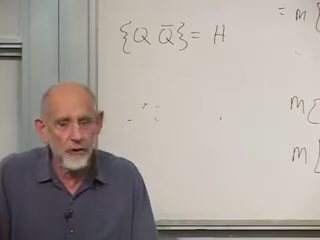
\includegraphics[width=0.62\textwidth]{lecture_05_figure_02.png}
\lectureframe{00:55:46.300}
\caption{Выделенное на доске центральное соотношение замыкания. Фигурные скобки и \(Q,\bar Q,H\) видны; запятая восстанавливается по стандартному обозначению антикоммутатора.}
\end{figure}

Аддитивный нуль энергии выбран так, что пустое состояние имеет \(H=0\). Для суперсимметричного осциллятора это естественное соглашение: бозонный и фермионный вклады нулевых колебаний взаимно сокращаются. \editorialnote{В лекции сразу используется полная энергия покоя и отдельно не выписываются члены нулевой энергии; указанное соглашение делает этот выбор явным.}

Гамильтониан чётен. Он также является генератором симметрии: он порождает сдвиги по времени. Поэтому нечётные генераторы не замыкаются между собой, если не включить чётный генератор временных сдвигов.

\begin{classroomqa}
\audiencequestion{Какой член этого соотношения чётный? Это гамильтониан? \lecturetimestamp{00:58:24}}
\lecturerresponse{Да. Энергия — обычная наблюдаемая величина, поэтому \(H\) чётен. Суперзаряд \(Q\) нечётен, а произведение двух нечётных величин чётно; соответственно, \(\{Q,\bar Q\}\) может равняться \(H\). Нечётный и чётный генераторы связаны коммутатором, а не антикоммутатором.}
\end{classroomqa}

\subsection{Завершение алгебры}

Соотношения для генераторов одинаковой чётности сразу очевидны:
\begin{equation}
\{Q,Q\}=2Q^2=0,
\qquad
\{\bar Q,\bar Q\}=2\bar Q^2=0,
\end{equation}
поскольку \(Q^2\) содержит \(c_-^2\), а \(\bar Q^2\) содержит \(c_+^2\).

Остаётся соотношение с \(H\). Пусть
\begin{equation}
H\ket{E}=E\ket{E}.
\end{equation}
Если массы бозона и фермиона равны, \(Q\) заменяет одну частицу другой, не изменяя энергии. Следовательно, \(Q\ket{E}\) либо равно нулю, либо является другим собственным состоянием с тем же собственным значением:
\begin{equation}
H Q\ket{E}=E Q\ket{E}.
\end{equation}
С другой стороны,
\begin{equation}
QH\ket{E}=Q(E\ket{E})=E Q\ket{E}.
\end{equation}
Вычитая,
\begin{equation}
[H,Q]\ket{E}=0.
\end{equation}
Если собственные состояния энергии образуют полный базис, то это верно как операторное тождество:
\begin{equation}
[H,Q]=0,
\qquad
[H,\bar Q]=0.
\end{equation}

\begin{classroomqa}
\audiencequestion{Что происходит, если массы бозона и фермиона не совпадают? \lecturetimestamp{01:01:16}}
\lecturerresponse{Тогда замена одного другим меняет энергию, так что предлагаемый суперзаряд не коммутирует с гамильтонианом, и простая суперсимметрия теряется. Для
\[
H=m_BN_B+m_FN_F,
\]
явный результат имеет вид
\[
[H,Q]=(m_B-m_F)Q.
\]
Он обращается в нуль в точности при \(m_B=m_F\). \editorialnote{Коммутатор при неравных массах есть прямая операторная форма аргумента об изменении энергии и делает условие равенства масс явным.}}
\end{classroomqa}

\begin{classroomqa}
\audiencequestion{Нельзя ли повторить аргумент с собственными состояниями энергии чуть медленнее? \lecturetimestamp{01:01:37}}
\lecturerresponse{Начнём с \(H\ket{E}=E\ket{E}\). Равенство масс влечёт, что \(Q\ket{E}\) имеет ту же определённую энергию \(E\), так что \(HQ\ket{E}=EQ\ket{E}\). В другом порядке получается \(QH\ket{E}=QE\ket{E}=EQ\ket{E}\), потому что \(E\) — обычный скаляр. Их разность обращается в нуль на каждом собственном состоянии энергии. Полнота затем переносит это утверждение с этих состояний на операторное уравнение \([H,Q]=0\).}
\end{classroomqa}

Итак, полная игрушечная алгебра имеет вид
\begin{align}
\{Q,\bar Q\}&=H,\\
\{Q,Q\}&=\{\bar Q,\bar Q\}=0,\\
[H,Q]&=[H,\bar Q]=0.
\end{align}
Суперзаряды являются сохраняющимися нечётными зарядами. Ещё более удивительно то, что их алгебра смешивает операцию, меняющую тип частицы, с генератором пространственно-временного сдвига.

\section{Почему гамильтониан является генератором сдвигов по времени}

В этой предельно упрощённой модели нет пространственной координаты, но есть время. Уравнение Шрёдингера имеет вид
\begin{equation}
i\frac{\partial}{\partial t}\ket{\psi(t)}
=H\ket{\psi(t)}.
\end{equation}

\begin{figure}[H]
\centering
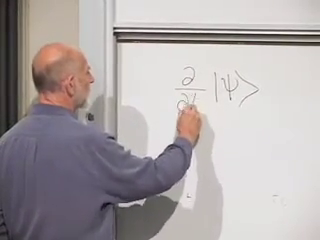
\includegraphics[width=0.56\textwidth]{lecture_05_figure_03.png}
\lectureframe{01:07:26.300}
\caption{Производная по времени записана рядом с \(\ket{\psi}\). Рука закрывает часть знаменателя; полное уравнение Шрёдингера приведено выше.}
\end{figure}

Для конечного сдвига \(\delta\),
\begin{equation}
\ket{\psi(t+\delta)}
=e^{-iH\delta}\ket{\psi(t)}.
\end{equation}
Разлагая по первому порядку,
\begin{equation}
\ket{\psi(t+\delta)}
=\left(\mathbf 1-i\delta H\right)\ket{\psi(t)}
+O(\delta^2).
\end{equation}
Таким образом, \(H\) — бесконечно малый генератор, сдвигающий состояние по времени.

Внутренние симметрии, такие как изоспин и цвет, тоже меняют метки частиц. Изоспин может смешивать состояния протона и нейтрона; цветовые вращения смешивают красные, зелёные и синие кварки. Однако никакая композиция этих внутренних преобразований не сдвигает систему в пространстве или во времени. С суперсимметрией дело обстоит иначе:
\begin{equation}
\begin{gathered}
\text{odd particle-changing transformation}\\
\mathrel{\stackrel{\{\ ,\ \}}{\Longrightarrow}}\\
\text{time translation}
\end{gathered}
\end{equation}
Это и есть указание на то, что нечётные генераторы сами могут быть сдвигами, но вдоль координат, отличных от обычных.

\section{Суперпространство}

\subsection{Функция времени и нечётных координат}

Введём функцию
\begin{equation}
\Psi=\Psi(\theta,\bar\theta,t).
\end{equation}
Её можно рассматривать как волновую функцию в игрушечной модели или, более общо, как суперполе. Поскольку разложение по нечётным координатам обрывается,
\begin{equation}
\Psi(\theta,\bar\theta,t)
=A(t)+\bar\chi(t)\theta
+\bar\theta\chi(t)+F(t)\bar\theta\theta.
\end{equation}
Этот единый объект объединяет в себе чётные и нечётные компонентные функции. \editorialnote{В этом компонентном разложении используется полином Грассмана, введённый ранее; это стандартное явное содержание функции на игрушечном суперпространстве.}

Обычный сдвиг по времени оставляет \(\theta,\bar\theta\) неизменными и переводит
\begin{equation}
t\longmapsto t+\delta.
\end{equation}
В первом порядке,
\begin{equation}
\Psi(\theta,\bar\theta,t+\delta)
=\Psi(\theta,\bar\theta,t)
+\delta\,\partial_t\Psi(\theta,\bar\theta,t).
\end{equation}

\begin{figure}[H]
\centering
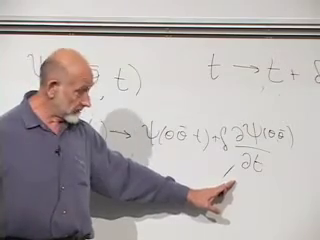
\includegraphics[width=0.72\textwidth]{lecture_05_figure_04.png}
\lectureframe{01:13:15.060}
\caption{На доске \(t\to t+\delta\) помещено над изменением \(\Psi\) в первом порядке, причём член с производной указан непосредственно.}
\end{figure}

\subsection{Сдвиг в нечётном направлении}

Теперь введём преобразование, сдвигающее нечётную координату:
\begin{equation}
\theta\longmapsto\theta+\epsilon,
\end{equation}
где \(\epsilon\) — ещё один нечётный параметр Грассмана. Одновременно пусть время получает чётное нильпотентное смещение,
\begin{equation}
t\longmapsto t+i\bar\theta\epsilon.
\end{equation}
И \(\bar\theta\), и \(\epsilon\) нечётны, так что их произведение чётно и его можно согласованно прибавить к чётной координате \(t\).

Перенеся параметр влево,
\begin{equation}
i\bar\theta\epsilon=-i\epsilon\bar\theta.
\end{equation}
Поэтому индуцированная вариация имеет вид
\begin{align}
\delta_\epsilon\Psi
&=\epsilon\,\partial_\theta\Psi
-i\epsilon\bar\theta\,\partial_t\Psi\\
&=\epsilon q_0\Psi,
\end{align}
где
\begin{equation}
q_0=\partial_\theta-i\bar\theta\partial_t.
\end{equation}
Этот нечётный дифференциальный оператор является генератором комбинированного сдвига. Совместимый сопряжённый генератор, использующий левые производные, имеет вид
\begin{equation}
\bar q_0=-\partial_{\bar\theta}
+i\theta\partial_t.
\end{equation}

Точные знаки зависят от того, используются ли левые или правые производные по Грассману и от того, как сопряжение обращает порядок нечётных множителей. То, что не должно зависеть от соглашения, — это замыкание на трансляцию по времени. При приведённых выше определениях,
\begin{align}
\{q_0,\bar q_0\}
&=i\{\partial_\theta,\theta\}\partial_t
+i\{\bar\theta,\partial_{\bar\theta}\}\partial_t\\
&=2i\partial_t.
\end{align}
Член с производными по двум переменным обращается в нуль, как и член, квадратичный по нечётным координатам. Два смешанных члена дают по \(i\partial_t\) каждый.

Поскольку для состояний в представлении Шрёдингера \(H=i\partial_t\),
\begin{equation}
\{q_0,\bar q_0\}=2H.
\end{equation}
Если ввести нормировку
\begin{equation}
q=\frac{q_0}{\sqrt2},
\qquad
\bar q=\frac{\bar q_0}{\sqrt2},
\end{equation}
то
\begin{equation}
\boxed{\{q,\bar q\}=H.}
\end{equation}
\editorialnote{В лекции намеренно проделывается вычисление с неуверенными знаками, а затем обнаруживается множитель два. Показанное соглашение с левыми производными сохраняет этот аудиторный расчёт, одновременно фиксируя одну самосогласованную нормировку. Другие стандартные соглашения перераспределяют знаки между сдвигами координат и генераторами.}

\begin{classroomqa}
\audiencequestion{Откуда берётся последний множитель два в антикоммутаторе суперпространства? \lecturetimestamp{01:24:21}}
\lecturerresponse{Есть два равных смешанных вклада. Один возникает из \(\{\partial_\theta,\theta\}=1\), а другой — из \(\{\partial_{\bar\theta},\bar\theta\}=1\). Каждый умножает производную по времени. Поэтому ненормированные генераторы дают \(2i\partial_t\); множитель \(1/\sqrt2\) в каждом суперзаряде восстанавливает прежнюю нормировку.}
\end{classroomqa}

\begin{classroomqa}
\audiencequestion{Использовалось ли в построении предположение, что \(\epsilon\) мало? \lecturetimestamp{01:24:51}}
\lecturerresponse{Использовалась нильпотентность, а не обычная численная малость. Поскольку \(\epsilon^2=0\), любое разложение по одной \(\epsilon\) обрывается после первого порядка. Называть этот параметр бесконечно малым или малым — полезная аналогия, но обрыв разложения точен.}
\end{classroomqa}

\editorialnote{Параметры Грассмана не имеют обычной положительной величины. Их роль бесконечно малых параметров обусловлена нильпотентностью и точным обрывом разложения.}

\subsection{Геометрический смысл}

Теперь эта алгебра имеет две эквивалентные реализации. В осцилляторной картине \(Q\) и \(\bar Q\) заменяют фермионы бозонами, а бозоны — фермионами. В геометрической картине \(q\) и \(\bar q\) сдвигают функцию по нечётным направлениям, вызывая при этом обычный сдвиг по времени. В обеих картинах,
\begin{equation}
\begin{gathered}
\{\text{supercharge},\text{conjugate supercharge}\}\\
=\text{time-translation generator}.
\end{gathered}
\end{equation}

Обобщённое координатное пространство, содержащее \(t,\theta,\bar\theta\), называется суперпространством. В релятивистской теории поля оно также содержит обычные пространственные координаты, и суперзаряды замыкаются на полный импульс пространства-времени \(P_\mu\), а не только на \(H=P_0\). Искривление этой структуры ведёт к супергравитации.

В одном смысле переменные Грассмана — это эффективное средство учёта бозонов и фермионов. В другом отношении соотношение замыкания говорит о гораздо более глубоком: различие между типом частицы и геометрией пространства-времени больше не является абсолютным. Двукратный сдвиг в нечётных направлениях порождает сдвиг в обычном направлении. Реализует ли природа такую структуру экспериментально, — отдельный вопрос по сравнению с математическим фактом, что эта структура внутренне согласована, экономна и поразительно жёстка.